\documentclass{article}

% packages
\usepackage{amsmath, amsthm, thmtools, amsfonts, amssymb, luacode, catchfile, tikzducks, hyperref, ifthen}
\ifcsname c@kobocompile\endcsname
	\usepackage[a5paper, total={1072pt, 1448pt}, margin=10pt, includeheadfoot]{geometry} % set page margins
\else
	\usepackage[a4paper, margin=50pt, includeheadfoot]{geometry}
\fi
\usepackage[shortlabels]{enumitem}
\usepackage[skip=3pt, indent=0pt]{parskip}

% language
\usepackage[bidi=basic, layout=tabular, provide=*]{babel}
\ifcsname c@english\endcsname
	\babelprovide[main, import]{english}
\else
	\babelprovide[main, import]{hebrew}
	\babelprovide{rl}
\fi
%\babelfont{rm}{Libertinus Serif}
\babelfont{rm}[Renderer=Harfbuzz]{Libertinus Serif}
\babelfont{sf}{Libertinus Sans}
\babelfont{tt}{Libertinus Mono}

% style
\AddToHook{cmd/section/before}{\clearpage}	% Add line break before section
\linespread{1.3}
\setcounter{secnumdepth}{0}		% Remove default number tags from sections, this won't do well with theorems
\AtBeginDocument{\setlength{\belowdisplayskip}{3pt}}
\AtBeginDocument{\setlength{\abovedisplayskip}{3pt}}
\graphicspath{ {../images/} }

% operators
\DeclareMathOperator\cis{cis}
\DeclareMathOperator\Sp{Sp}
\DeclareMathOperator\tr{tr}
\DeclareMathOperator\im{Im}
\DeclareMathOperator\re{Re}
\DeclareMathOperator\diag{diag}
\DeclareMathOperator*\lowlim{\underline{lim}}
\DeclareMathOperator*\uplim{\overline{lim}}
\DeclareMathOperator\rng{rng}
\DeclareMathOperator\Sym{Sym}
\DeclareMathOperator\Arg{Arg}
\DeclareMathOperator\Log{Log}
\DeclareMathOperator\dom{dom}
\DeclareMathOperator\supp{Supp}
\DeclareMathOperator\var{Var}
\DeclareMathOperator\cov{Cov}

% commands
%\renewcommand\qedsymbol{\textbf{מש''ל}}
%\renewcommand\qedsymbol{\fbox{\emoji{lizard}}}
\newcommand{\Aa}[0]{\mathcal{A}}
\newcommand{\Bb}[0]{\mathcal{B}}
\newcommand{\CC}[0]{\mathbb{C}}
\newcommand{\Cc}[0]{\mathcal{C}}
\newcommand{\EE}[0]{\mathbb{E}}
\newcommand{\FF}[0]{\mathbb{F}}
\newcommand{\Ff}[0]{\mathcal{F}}
\newcommand{\Ii}[0]{\mathcal{I}}
\newcommand{\Gg}[0]{\mathcal{G}}
\newcommand{\Ll}[0]{\mathcal{L}}
\newcommand{\Mm}[0]{\mathcal{M}}
\newcommand{\NN}[0]{\mathbb{N}}
\newcommand{\Nn}[0]{\mathcal{N}}
\newcommand{\PP}[0]{\mathbb{P}}
\newcommand{\Pp}[0]{\mathcal{P}}
\newcommand{\QQ}[0]{\mathbb{Q}}
\newcommand{\RR}[0]{\mathbb{R}}
\newcommand{\Rr}[0]{\mathcal{R}}
\newcommand{\Ss}[0]{\mathcal{S}}
\newcommand{\TT}[0]{\mathbb{T}}
\newcommand{\Uu}[0]{\mathcal{U}}
\newcommand{\Vv}[0]{\mathcal{V}}
\newcommand{\Ww}[0]{\mathcal{W}}
\newcommand{\ZZ}[0]{\mathbb{Z}}
\newcommand{\acts}[0]{\circlearrowright}
\newcommand{\explain}[2] {
	\begin{flalign*}
		 && \text{#2} && \text{#1}
	\end{flalign*}
}
\newcommand{\maketitleprint}[0]{ \begin{center}
	%\begin{tikzpicture}[scale=3]
	%	\duck[graduate=gray!20!black, tassel=red!70!black]
	%\end{tikzpicture}	
	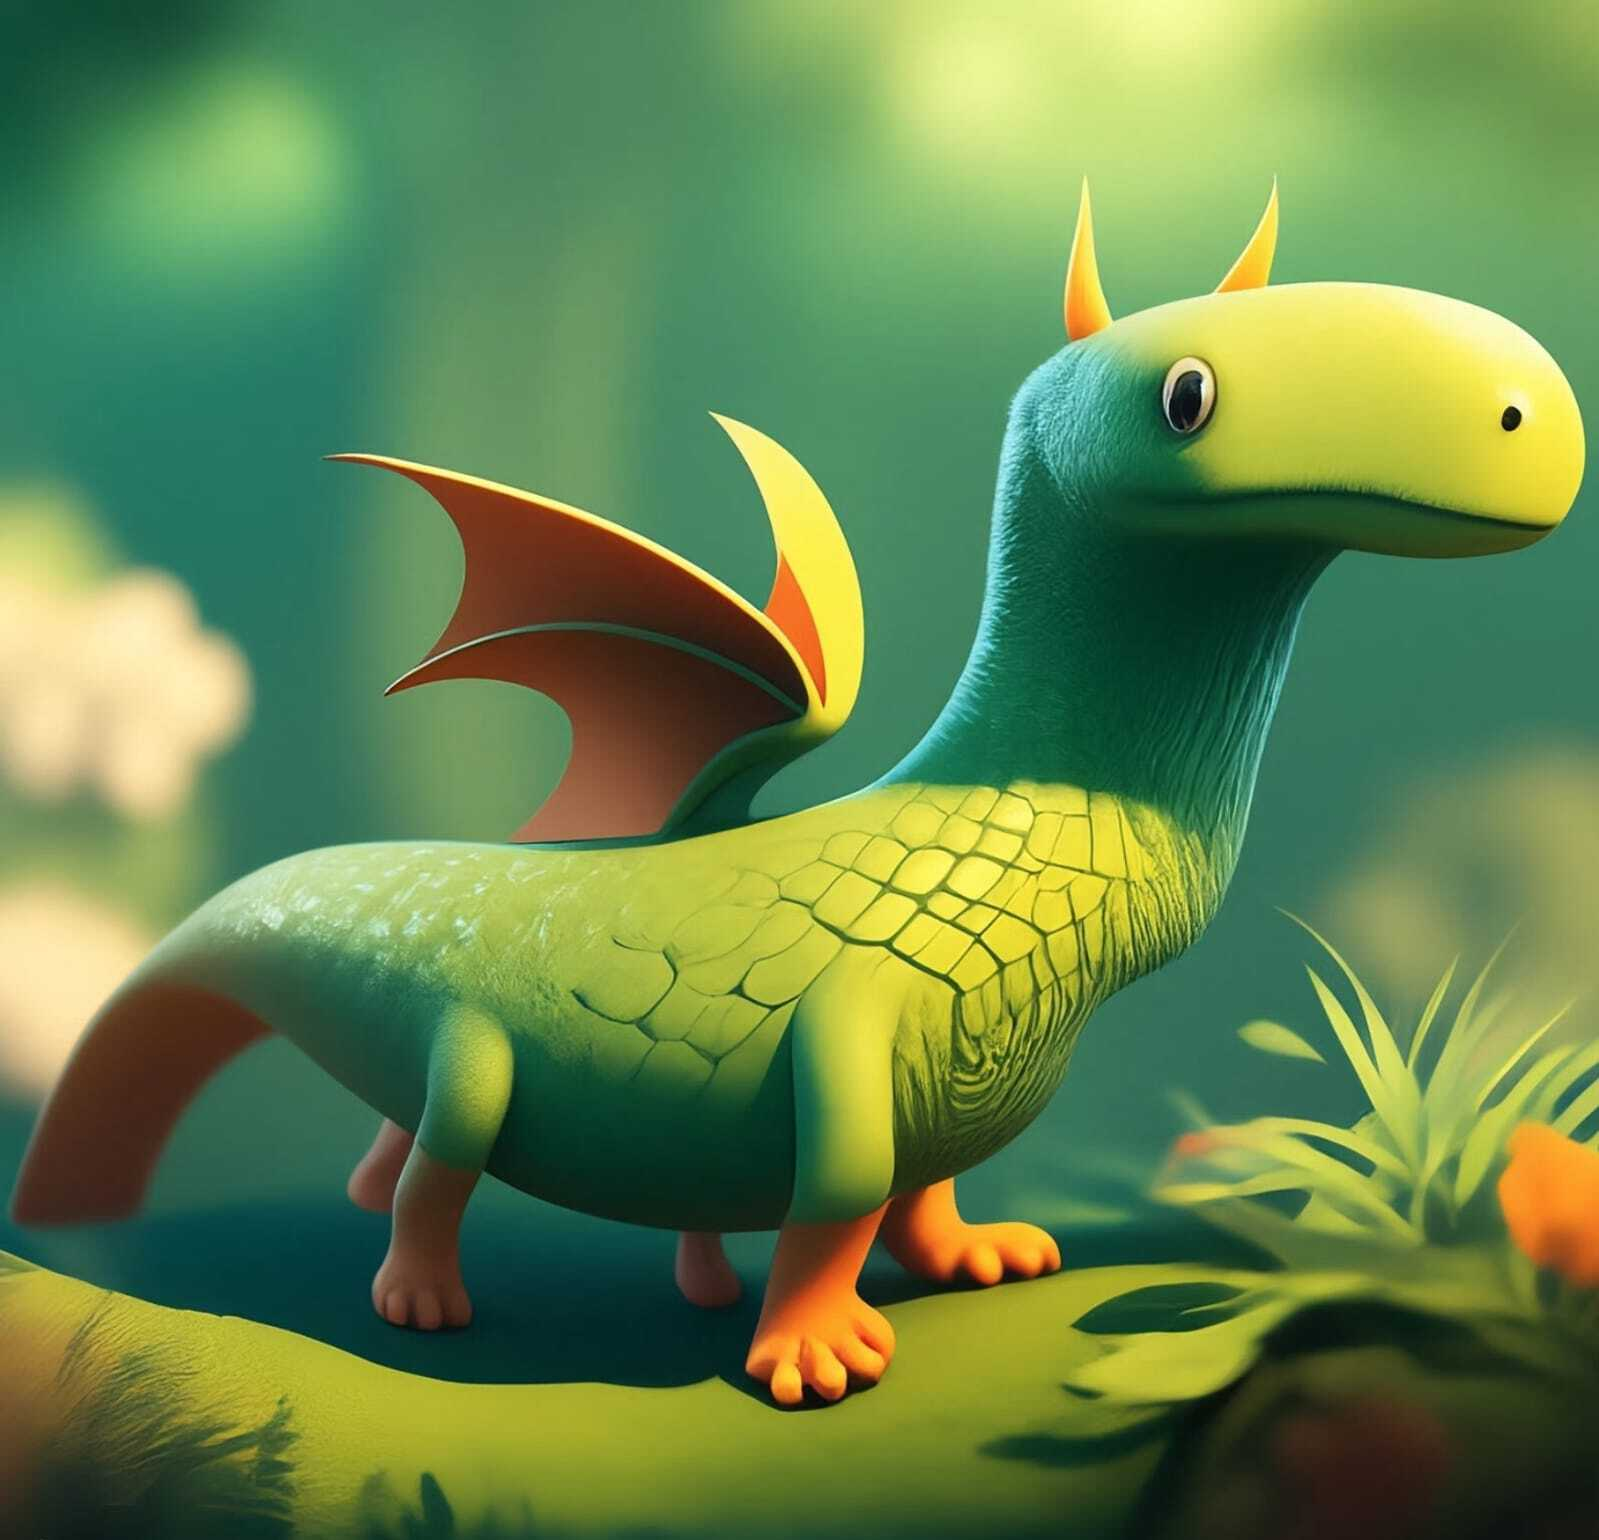
\includegraphics[width=6cm]{cover}
\end{center}
}

% theorem commands
\newtheoremstyle{c_remark}
	{}	% Space above
	{}	% Space below
	{}% Body font
	{}	% Indent amount
	{\bfseries}	% Theorem head font
	{}	% Punctuation after theorem head
	{.5em}	% Space after theorem head
	{\thmname{#1}\thmnumber{ #2}\thmnote{ \normalfont{\text{(#3)}}}}	% head content
\newtheoremstyle{c_definition}
	{3pt}	% Space above
	{3pt}	% Space below
	{}% Body font
	{}	% Indent amount
	{\bfseries}	% Theorem head font
	{}	% Punctuation after theorem head
	{.5em}	% Space after theorem head
	{\thmname{#1}\thmnumber{ #2}\thmnote{ \normalfont{\text{(#3)}}}}	% head content
\newtheoremstyle{c_plain}
	{3pt}	% Space above
	{3pt}	% Space below
	{\itshape}% Body font
	{}	% Indent amount
	{\bfseries}	% Theorem head font
	{}	% Punctuation after theorem head
	{.5em}	% Space after theorem head
	{\thmname{#1}\thmnumber{ #2}\thmnote{ \text{(#3)}}}	% head content

\ifcsname c@english\endcsname
	\theoremstyle{plain}
	\newtheorem{theorem}{Theorem}[section]
	\newtheorem{lemma}[theorem]{Lemma}
	\newtheorem{proposition}[theorem]{Proposition}
	\newtheorem*{proposition*}{Proposition}
	%\newtheorem{corollary}[theorem]{אין חלופה עברית}

	\theoremstyle{definition}
	\newtheorem{definition}[theorem]{Definition}
	\newtheorem*{definition*}{Definition}
	\newtheorem{example}{Example}[section]
	\newtheorem{exercise}{Exercise}[section]

	\theoremstyle{remark}
	\newtheorem*{remark}{Remark}
	\newtheorem*{solution}{Solution}
	\newtheorem{conclusion}[theorem]{Conclusion}
	\newtheorem{notation}[theorem]{Notation}
\else
	\theoremstyle{c_plain}
	\newtheorem{theorem}{משפט}[section]
	\newtheorem{lemma}[theorem]{למה}
	\newtheorem{proposition}[theorem]{טענה}
	\newtheorem*{proposition*}{טענה}
	%\newtheorem{corollary}[theorem]{אין חלופה עברית}

	\theoremstyle{c_definition}
	\newtheorem{definition}[theorem]{הגדרה}
	\newtheorem*{definition*}{הגדרה}
	\newtheorem{example}{דוגמה}[section]
	\newtheorem{exercise}{תרגיל}[section]

	\theoremstyle{c_remark}
	\newtheorem*{remark}{הערה}
	\newtheorem*{solution}{פתרון}
	\newtheorem{conclusion}[theorem]{מסקנה}
	\newtheorem{notation}[theorem]{סימון}
\fi

% Questions related commands
\newcounter{question}
\setcounter{question}{1}
\newcounter{sub_question}
\setcounter{sub_question}{1}

\ifcsname c@english\endcsname
	\newcommand{\question}[1][0]{
		\ifthenelse{#1 = 0}{}{\setcounter{question}{#1}}
		\section{Question \arabic{question}}
		\addtocounter{question}{1}
		\setcounter{sub_question}{1}
	}

	\newcommand{\subquestion}[1][0]{
		\ifthenelse{#1 = 0}{}{\setcounter{sub_question}{#1}}
		\subsection{Part \alph{sub_question}}
		\addtocounter{sub_question}{1}
	}
\else
	\newcommand{\question}[1][0]{
		\ifthenelse{#1 = 0}{}{\setcounter{question}{#1}}
		\section{שאלה \arabic{question}}
		\addtocounter{question}{1}
		\setcounter{sub_question}{1}
	}

	\newcommand{\subquestion}[1][0]{
		\ifthenelse{#1 = 0}{}{\setcounter{sub_question}{#1}}
		\subsection{סעיף \localecounter{letters.gershayim}{sub_question}}
		\addtocounter{sub_question}{1}
	}
\fi

% import lua and start of document
\directlua{common = require ('../common')}

\GetEnv{AUTHOR}

% headers
\author{\AUTHOR}
\date\today

\title{פתרון מטלה 03 --- מבנים אלגבריים (2), 80446}

\begin{document}
\maketitle
\maketitleprint[red]

\question{}
תהי $L / F$ הרחבת שדות ויהיו $g, h \in F[x]$.
נראה ש־$\gcd_{L[x]}(g, h) = \gcd_{F[x]}(g, h)$, כלומר נראה ש־$\gcd$ נשמר תחת הרחבת שדות.
\begin{proof}
	נניח ש־$f = \gcd_{F[x]}(g, h)$.
	נניח גם ש־$\overline{f} = \gcd_{L[x]}(g, h)$.
	כל פולינום $l \in F[x]$ הוא בפרט פולינום גם ב־$L[x]$ ולכן אם $l \mid g, h$ אז $\overline{f} \mid l$, אז בפרט גם $\overline{f} \mid f$ במקרה של $l = f$.

	המעלה של $\overline{f}$ קטנה משל $f$, אחרת ניקח את החיסור שלהם כשהם מתוקנים ונקבל פולינום קטן יותר שמחלק את $g, h$.
	נניח ש־$f = q \overline{f} + r$.
	אם $q, r \in F[x]$ אז $\overline{f} \in F[x]$ ונסיק ש־$f = \overline{f}$.
	נניח אם כך אחרת, אילו $q \in F[x]$ אבל $r \notin F[x]$ אז נקבל ש־$r = q \overline{f} - f \in F[x]$ וקיבלנו סתירה.
	נניח ש־$q \notin F[x]$.

	יהי $\alpha x^i$ מונום המרכיב את $q$ המעיד על $l \notin F[x]$, כלומר $\alpha \in L \setminus F$, ונניח גם כי זהו המונום הגדול ביותר המעיד על־כך, דהינו אם קיים $\beta x^j$ כך שגם $\beta \notin F$ ו־$j > i$, אז נבחר אותם במקום.
	לכל $a \in F$, אנו יודעים ש־$a + \alpha, a \cdot \alpha \notin F$, כהיסק מסגירות הכפל לפעולות אלה.
	נניח בלי הגבלת הכלליות ש־$f, \overline{f}$ מתוקנים שניהם.
	נבחין כי הדרגה של $r$ קטנה מזו של $q \cdot \overline{f}$, וכן נבחין ש־$\alpha x^i x^n$ עבור $n = \deg \overline{f}$ הוא מונום של $q \overline{f}$, ומהגדרת $r$ אין לו איברים מסדר $i + n$.
	נקבל אם כך ש־$q \cdot \overline{f} \notin F[x]$ וגם ש־$q \overline{f} + r \notin F[x]$, אבל זו סתירה כי $q \overline{f} + r = f \in F[x]$.
	
	קיבלנו ש־$q, r \in F[x]$ ולכן בפרט $f = \overline{f}$.
\end{proof}

\question{}
יהי $F$ שדה.

\subquestion{}
יהי $c \in F$ ויהיו $g, h \in F[x]$.

\subsubsection{i}
נראה ש־${(g + h)}' = g' + h'$.
\begin{proof}
	נניח ש־$g = \sum_{i = 0}^n \alpha_i x^i$ וכן ש־$h = \sum_{i = 0}^n \beta_i x^i$, עבור $\alpha_i, \beta_i \in F$, $n \in \NN$.
	נבחין כי אם דרגות הפולינומים לא שוות, אז $\alpha_i = 0$ או $\beta_i = 0$ החל מ־$i$ כלשהו, אך אין משמעות לעובדה זו בחישוב.
	עתה נבדוק את הזהות,
	\[
		(g + h)'
		= \sum_{i = 1}^n i (\alpha_i + \beta_i) x^{i - 1}
		= \sum_{i = 1}^n i \alpha_i x^{i - 1} + \sum_{i = 1}^n i \beta_i x^{i - 1}
		= g' + h'
	\]
	ולכן הזהות אכן חלה.
\end{proof}

\subsubsection{ii}
נראה ש־$(c \cdot g)' = c \cdot g'$.
\begin{proof}
	נבדוק,
	\[
		(c \cdot g)'
		= \left( c \cdot \sum_{i = 0}^n \alpha_i x^i \right)'
		= \left( \sum_{i = 0}^n c \alpha_i x^i \right)'
		= \sum_{i = 1}^n i c \alpha_i x^{i - 1}
		= c \sum_{i = 1}^n i \alpha_i x^{i - 1}
		= c \cdot g'
	\]
	וקיבלנו שאכן הזהות מתקיימת.
\end{proof}

\subsubsection{iii}
נראה שמתקיים, $(g \cdot h)' = g' \cdot h + g \cdot h'$.
\begin{proof}
	\begin{align*}
		(g \cdot h)'
		& = \left( g \cdot \sum_{i = 0}^n \beta_i x^i \right)' \\
		& = \left( \sum_{i = 0}^n g \cdot \beta_i x^i \right)' \\
		& = \sum_{i = 0}^n \beta_i (g \cdot x^i)' \\
		& = \sum_{i = 0}^n \beta_i \sum_{j = 1}^n \alpha_j (i + j) x^{i + j - 1} \\
		& = \sum_{i = 0}^n \beta_i \left( i x^{i - 1} \sum_{j = 1}^n \alpha_j x^j + x^i \sum_{j = 1}^n \alpha_j j x^{j - 1} \right) \\
		& = \sum_{i = 0}^n \beta_i \left( i x^{i - 1} g + x^i g' \right) \\
		& = g \sum_{i = 0}^n \beta_i i x^{i - 1} + g' \sum_{i = 0}^n \beta_i x^i \\
		& = g h' + g' h
	\end{align*}
\end{proof}

\subquestion{}
נוכיח את המקרה הפרטי לכלל לופיטל,
אם $a \in F$ שורש של $g \in F[x]$ כך ש־$g(x) = h(x) \cdot (x - a)$, אז $g'(a) = h(a)$.
\begin{proof}
	מתקיים,
	\[
		g'(x)
		= h'(x) (x - a) + h(x)
	\]
	מהזהויות שמצאנו בסעיף הקודם.
	נציב ונקבל,
	\[
		g'(a)
		= h'(a) (a - a) + h(a)
		= h(a)
	\]
	ומצאנו כי אכן מתקיים השוויון שרצינו להראות.
\end{proof}

\question{}
בכל סעיף נגדיר פולינום ונבדוק אם הוא ספרבילי מעל $\QQ$, נמצא שורשים מריבוי גדול מאחד.

\subquestion{}
נגדיר $f(x) = x^3 - 3x + 2$.
\begin{solution}
	נבחין כי $f(x) = {(x - 1)}^2 (x + 2)$ מחלוקת פולינומים והעובדה ש־$f(1) = 0$.
	לכן נסיק שהפולינום הוא לא ספרבילי וש־$1$ שורש כפול.
\end{solution}

\subquestion{}
נגדיר $f(x) = x^3 - 7x + 6$.
\begin{solution}
	עלינו לבדוק את $x = \pm 1, \pm 2, \pm 3$,
	נקבל מחישוב ש־$f(2) = 0$, ומחילוק פולינומים נקבל,
	\[
		f(x)
		= (x - 1) (x - 2) (x + 3)
	\]
	ולכן הפולינום הוא ספרבילי.
\end{solution}

\subquestion{}
נגדיר $f(x) = x^4 - 4x^3 + 6x^2 - 4x + 1$.
\begin{solution}
	הפעם עלינו לבדוק את $x = \pm 1$ בלבד, ונקבל $f(1) = 0$.
	מחלוקת פולינומים נקבל $f(x) = (x - 1)(x^3 - 3x^2 + 3x - 1) = {(x - 1)}^4$.
	נסיק אם כך שהפולינום לא ספרבילי והריבוי של $x = 1$ הוא $4$.
\end{solution}

\question{}


\end{document}
